\documentclass[tikz,border=2pt]{standalone}
\usepackage{amsmath,amssymb}
\usetikzlibrary{arrows.meta}

\begin{document}
% Topologist's sine curve: {(0,0)} together with the graph of sin(1/x) for x > 0. The graph
% oscillates ever faster as x -> 0+, so no path inside the set reaches (0,0).
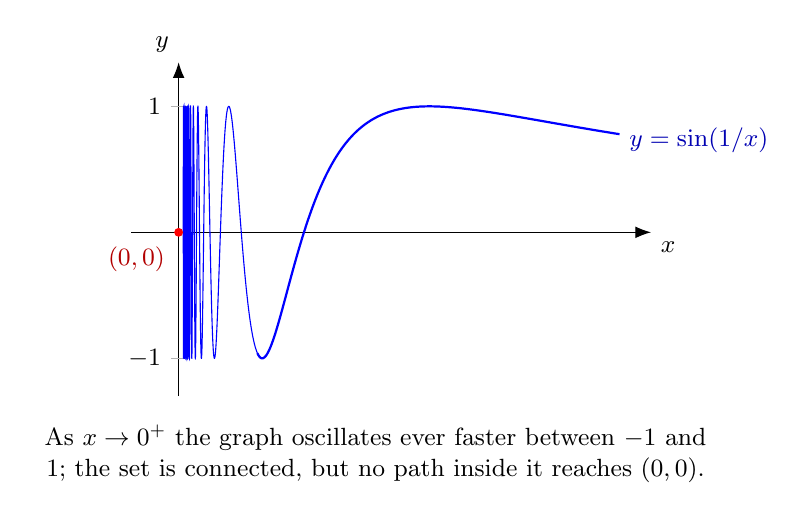
\begin{tikzpicture}[every node/.style={font=\small}, >={Latex[length=2mm]}, x=5cm, y=1.6cm]
	\draw[->] (-0.12,0) -- (1.2,0) node[below right] {$x$};
	\draw[->] (0,-1.3) -- (0,1.35) node[above left] {$y$};
	\draw[gray!60] (-0.02,1) -- (0.02,1) node[pos=0, left, font=\small, text=black] {$1$};
	\draw[gray!60] (-0.02,-1) -- (0.02,-1) node[pos=0, left, font=\small, text=black] {$-1$};
	% Sampled in t = 1/x: TikZ's fixed-point steps in x are too coarse near 0.
	\draw[blue, thin, variable=\t, domain=5:85, samples=3000] plot ({1/\t},{sin(deg(\t))});
	\draw[blue, thick, variable=\t, domain=0.893:5, samples=300] plot ({1/\t},{sin(deg(\t))});
	\fill[red] (0,0) circle (1.6pt);
	\node[red!70!black, anchor=north east, font=\small] at (-0.01,-0.04) {$(0,0)$};
	\node[blue!70!black, anchor=west, font=\small] at (1.12,0.73) {$y=\sin(1/x)$};
	\node[anchor=north, align=flush center, text width=8.6cm] at (0.5,-1.45) {As $x\to0^+$ the graph oscillates ever faster between $-1$ and $1$; the set is connected, but no path inside it reaches $(0,0)$.};
\end{tikzpicture}
\end{document}
